\chapter{Recursion}\label{ch:recursion}

Recrusion is a very upper level categorization of problems, in the function call itself for either or more than one times.

\marginnote{Calling more than one time? $\Rightarrow$ memoization can be used to save time.}

There are various \textbf{algorithm paradigm} which usages recursion.

\rule{\textwidth}{1.5pt}
Recursion Observations:
\begin{description}
    \item [Backtracking:] Backtracking problem are the one in which we browse the state-space-tree using recursion.
    \item [Branch and Bound:] Backtraking explores the state-space-tree in DFS manner, where Branch and Bound explores the state-space-tree in BFS manner.(using queue,stack or priorityqueue)
    
    \item [One-Time-Recursion:] In these type of problems , the subproblem computation are used \textbf{exactly once}. Hence no need to memoize the computation.
    List of problems paradigm having no need of memoization are:
    \begin{description}
        \item [Binary Search:] find element, find lowerbound, find upperbound, find inflection point.
        \item [Quick sort:] Quick Sort Algorithm, Number of inversion in quick sort.
        \item [Divide and Conquere:] Merge Sort, 
        \item [Union Find:] union find class, union by rank, path compression.
        \item [Graph Traversal and Graph Algorithm:] (ex: DFS,Topological)
        \item [Tree Traversal and Tree Algorithms:]
        \item [Trie Algorithms:]
    \end{description}

    All of the above usages recursion in their implementation, but none of them require to require to re-use the computed result.

    TO-DO: Add 2,3 image summary showing code of all of above recursion.

    \item [DP Without State Change:] DP problem are the one in which same subproblem can be called multiple times. Hence we need to memoize the subproblem result.
    \begin{marginfigure}
        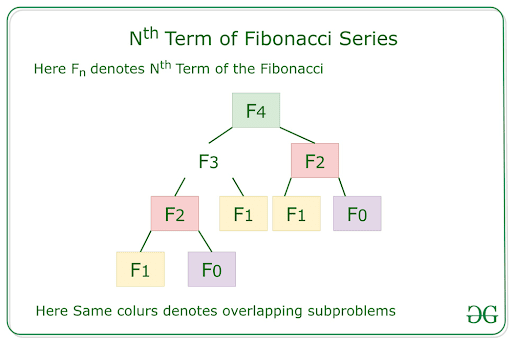
\includegraphics[width=\marginparwidth]{resources/fibonnaci_repeated_computation.png}
        \caption{Repeated use of Fibbonaci(2) in the recursion-tree.}
    \end{marginfigure}

    In dp recursive problem, the problem is divided into similar smaller problem, and then recursion is called on them.

    Example Problems: Coin Change, all classic dp problems.

    \item [DP with State Change:] Similar to backtracking, but ideally the state change is seperated from input and can be memoize seperately.
    
    Example Problems: No of ways to Paint, Stock Problem Series on LC, LC1349(Maximum Student taking exam), smallest team(LC1125), etc.
\end{description}

\vspace{2cm}
Backtracking vs Dynamic Programming:

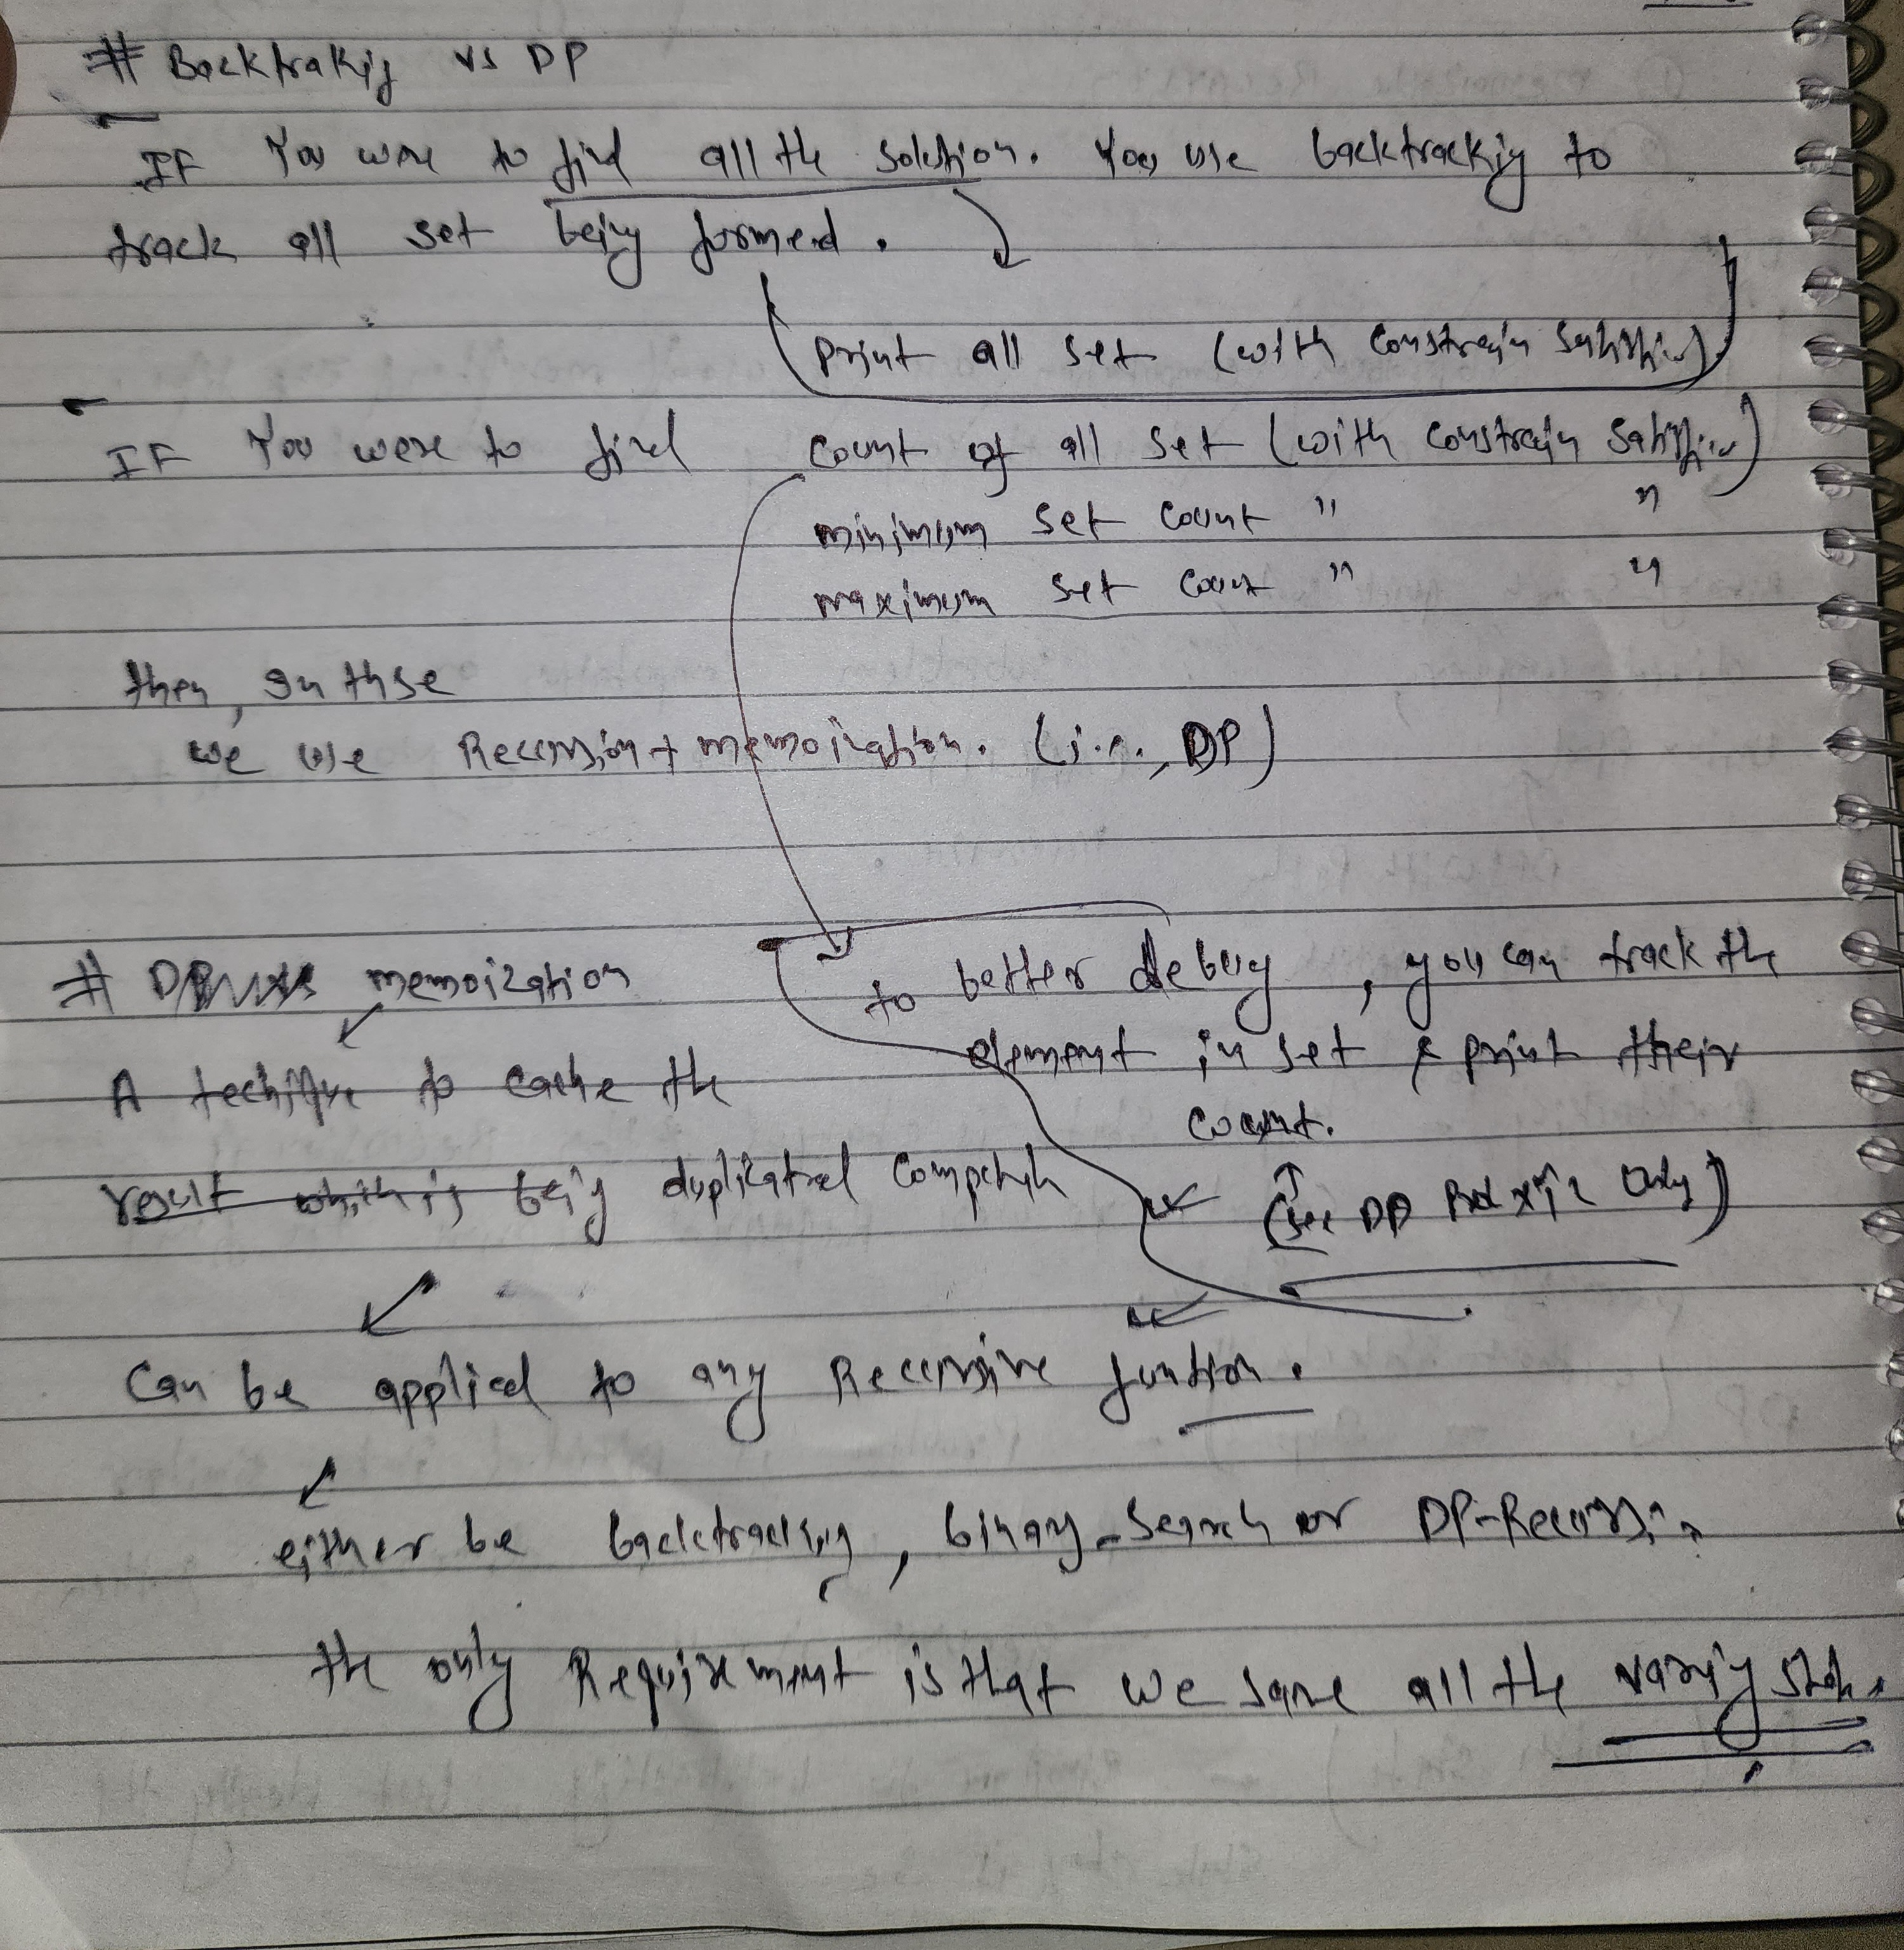
\includegraphics[width=\textwidth]{resources/backtrackingvsdp.jpg}

\rule{\textwidth}{1pt}








% All list of algoritm paradigm:
% \begin{compactenum}
%     \item Binary Search
%     \item Divide and Conquere
%     \item Graph
% \end{compactenum}
